\chapter{Mathe}
\section{Grundlagen}
\subsection{Mengen}
\bla{Mengen Darstellung}

\noindent\begin{tabularx}{\textwidth}{lX}

\toprule
 Schreibweise & Bedeutung \\
\midrule
$a \in M:$ & a ist ein Element von M \\
$a \not \in M:$ & a ist kein Element von M \\
$M=\{x | x \text{ Eigenschaften},\ldots\}$ & Beschreibende Darstellung \\
$M=\{a_1,a_2\ldots,a_n\}$ &Aufzählende Darstellung(endlich) \\
$M=\{a_1,a_2\ldots\}$ & Aufzählende Darstellung(unendlich) \\
$M=\{\}$ &Leere Menge \\
$A\subset B$ & A ist eine \emph{Teilmenge} von B. A heißt \emph{Untermenge} und B \emph{Obermenge}\\
$A=B$ & A und B sind gleich, d.h. jedes Element von A ist auch in B vorhanden und umgekehrt\\
\bottomrule
\end{tabularx}

\bla{Mengen Operationen}

\noindent\begin{tabularx}{\textwidth}{lX}
\toprule
 Schreibweise & Bedeutung \\
\midrule
$A\cap B=\{x|x\in A \text{ und } x\in B$ & \emph{Schnittmenge} zweier Mengen \\
$A\cup B=\{x|x\in A \text{ oder } x\in B\}$ & \emph{Vereinigungsmenge} zweier Mengen \\
$A\setminus B=\{x|x\in A \text{ und } x\not \in B\}$ & \emph{Differenz- oder Restmenge} zweier Mengen \\
\bottomrule
\end{tabularx}


\subsection{Intervalle}

\begin{tabularx}{\textwidth}{p{4cm}X}
\toprule
 Beispiel & Beschreibung \\
\midrule
\noindent
$[a,b]={x|a\leq x\leq b}$ & abgeschlossene Intervalle \\
$[a,b)={x|a\leq x < b}$ & halboffene Intervall\\
$(a,b]={x|a< x \leq b}$ & halboffene Intervall\\
$(a,b)={x|a<x<b}$ & offenes Intervall\\
\bottomrule
\end{tabularx}

\subsection{Rechnengesetze}

 \bla{Operationen mit Natürlichen Zahlen}
\begin{tabularx}{\textwidth}{p{3cm}X}
\toprule
 Beispiel & Beschreibung \\
\midrule
{\begin{align*}60 & =2^2\cdot3^1\cdot5^1 \\ 70 & =2^3\cdot3^2\\\text{ggt} & = 2^2\cdot3^1\end{align*}} & Zerlegung der Faktoren in ihre Primfaktoren und dann bildet man das Produkt aus denn höchsten Potenzen die alle Faktoren gemeinsam haben. \\
{\begin{align*}60 & =2^2\cdot3^1\cdot5^1 \\ 70 & =2^3\cdot3^2\\\text{kgV} & = 2^3\cdot3^2\cdot5^1\end{align*}}  &
Zerlegung der Faktoren in ihre Primfaktoren und dann bildet man das Produkt aus denn höchsten Potenzen die in mindestens einen Faktoren auftreten. \\
\bottomrule
\end{tabularx}

\bla{Kommutativgesetz}
\begin{shaded}
\begin{equation} \begin{split} a+b&=b+a\\a\cdot b&=b\cdot a \end{split} \end{equation} 
\end{shaded}
\bla{Assoziativgesetz}
\begin{shaded}
 

\begin{equation} \begin{split}a+(b+c) &=(a+b)+c\\a\cdot(b\cdot c)&=(a\cdot b)\cdot c\end{split} \end{equation}
\end{shaded}
\bla{Distributivgesetz}
 \begin{shaded}
\begin{equation} \begin{split}a\cdot(b+c)&=a\cdot b+a\cdot c\end{split}  \end{equation}
\end{shaded}

\subsection{Bruchrechnung}
Ein Bruch $a/b$ heißt \emph{echte}, wenn $|a|<|b|$ ist, sonst \emph{unecht}.

\bla{Addition und Subtraktion zweier Brüche}
\begin{shaded}
\begin{equation}
 \frac{a}{b}\pm\frac{c}{d}=\frac{a\cdot d \pm b\cdot c}{b\cdot d}
\end{equation}
\end{shaded}

\bla{Multiplikation zweier Brüche}
\begin{shaded}
\begin{equation}
 \frac{a}{b}\cdot\frac{c}{d}=\frac{a\cdot c}{b\cdot d}
\end{equation}
\end{shaded}
\bla{Division zweier Brüche}
\begin{shaded}
\begin{equation}
 \frac{a}{b}\div\frac{c}{d}=\frac{a\cdot d}{b\cdot c}
\end{equation}
\end{shaded}

\subsection{Potenzen}
Eine Potenz $a^n$ ist ein Produkt aus n gleichen Faktoren a:
\begin{shaded}
\begin{equation}
 a^n=a\cdot a \cdot a \ldots a
\end{equation}
$a:\text{ Basis}$ $n:\text{ Exponent}$
\end{shaded}
\bla{Rechenregeln}
\begin{shaded}
\begin{subequations}
\begin{equation}
 a^m*a^n=a^{m+n}
\end{equation}
\begin{equation}
\frac{a^m}{a^n}=a^{m-n}
\end{equation} 
\begin{equation}
 \left(a^m\right)^n=a^{m\cdot n}
\end{equation} 
\begin{equation}
 a^n\cdot b^n =\left(a\cdot b\right)^n
\end{equation} 
\begin{equation}
 \frac{a^n}{b^n}=\left(\frac{a}{b}\right)^n
\end{equation}
\end{subequations}
\end{shaded}
\subsection{Wurzeln}
Wurzelziehen ist die Umkehrfunktion des Potenzieren
\begin{shaded}
 \begin{equation}
\sqrt[n]{a}=a^{\left(\frac{1}{n}\right)}
\end{equation}
$a:\text{ Radikand}$ $n:\text{ Wurzelexponent}$  
\end{shaded}
\bla{Rechenregeln}
\begin{shaded}
\begin{subequations}
\begin{equation}
 \sqrt[n]{a^m}=a^{\left(\frac{m}{n}\right)}
\end{equation} 
\begin{equation}
 \sqrt[m]{\sqrt[n]{a}}=a^{\frac{1}{m\cdot n}}=\sqrt[m\cdot n]{a}
\end{equation} 
\begin{equation}
 \sqrt[n]{a}\cdot\sqrt[n]{b}=\sqrt[n]{a\cdot b}
\end{equation} 
\begin{equation}
 \frac{\sqrt[n]{a}}{\sqrt[n]{b}}=\sqrt[n]{\frac{a}{b}}
\end{equation} 
\end{subequations}
\end{shaded}

\subsection{Logarithmen}
Logarthmus ist das eindeutige lösen der Gleichung $r=a^x$ zur Lösung $x$.
\begin{shaded}
 \begin{equation}
  x=\log_{a}{r}
 \end{equation}
$a:\text{ Basis }(a>0,a\neq1)$ $r:\text{ Numerus }(r>0)$
\end{shaded}

\bla{Rechenregeln}
\begin{shaded}
\begin{subequations}
\begin{equation}
 \log_a b=\frac{\ln b}{\ln a}
\end{equation} 
\begin{equation}
 \log_a(u\cdot v) =\log_a u+\log_a v
\end{equation} 
\begin{equation}
 \log_a\left(\frac{u}{v}\right)=log_a u - \log_a v
\end{equation} 
\begin{equation}
 \log_a\left(u^k\right)=k\cdot\log_a u
\end{equation} 
\begin{equation}
 \log_a\sqrt[n]{u}=\left(\frac{1}{n}\right)\cdot\log_a u
\end{equation} 
\end{subequations}
\end{shaded}
\bla{Basiswechsel}
\begin{shaded}
 \begin{equation}
  \log_b r=\frac{\log_a r}{\log_a b}=\frac{1}{\log_a b}\cdot\log_a r =K\cdot\log_a r
 \end{equation}
\end{shaded}
Beim Basiswechsel von $a\rightarrow b$ werden die Logarithmen mit einer Konstanten K multipliziert.
\begin{shaded}
 \begin{align}
  \lg \rightarrow \ln \Rightarrow K&=2,3026 \\
  \ln \rightarrow \lg \Rightarrow K&=0,4343
 \end{align}
\end{shaded}

\subsection{Winkelfunktionen}
\begin{minipage}{.5\textwidth}
 \begin{shaded}\begin{align}
\sin{\alpha} &=\frac{a}{c}\\
\cos{\alpha} &=\frac{b}{c}\\
\tan{\alpha} &=\frac{a}{b}\\
\cot{\alpha} &=\frac{b}{a}
\end{align}
\end{shaded}
\end{minipage}\begin{minipage}{.5\textwidth}\begin{center} 
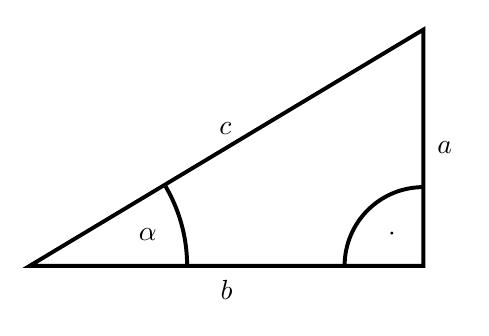
\begin{tikzpicture}[line width=.5mm]
%Dreieck
 \draw (0,0)--++(0:5cm)--++(90:3cm)--cycle;
\draw (2cm,0) arc (0:30.96:2cm);
\draw (4cm,0) arc (180:90:1cm);
%Deschriftung
\draw (4.6cm,.4)node{$\cdot$};
\draw (1.5cm,.4cm)node{$\alpha$};
\draw (5cm,1.5cm)node[right=1pt]{$a$};
\draw (2.5cm,0cm)node[below=1pt]{$b$};
\draw (30.96:2.9cm)node[above=1pt]{$c$};
\end{tikzpicture}
\end{center}
\end{minipage}

\bla{Rechenregeln}
\begin{shaded}
 \begin{align}
  \cos x &=\sin\left(x+\frac{\pi}{2}\right)&   \sin x &=\cos\left(x+\frac{\pi}{2}\right) \\
  \tan x &=\frac{\sin x}{\cos x}=\frac{1}{\cot x}& \cot x &=\frac{\cos x}{\sin x}=\frac{1}{\tan x}
\end{align}
\end{shaded}

\bla{Trigonometrischer Pythagoras}
\begin{shaded}
  \begin{equation}
\sin^2 x+ \cos^2 x =1
  \end{equation}
\end{shaded}

\bla{Addition von Winkeln}
\begin{shaded}
\begin{subequations}
  \begin{equation}
\sin\left(x_1\pm x_2\right)= \sin x_1 \cdot \cos x_2\pm \cos x_1 \cdot \sin x_2
  \end{equation}
  \begin{equation}
\cos\left(x_1\pm x_2\right)= \cos x_1 \cdot \cos x_2\mp \sin x_1 \cdot \sin x_2
  \end{equation}
  \begin{equation}
\tan\left(x_1\pm x_2\right)=\frac{\tan x_1 \pm \tan x_2}{1 \mp \tan x_1 \cdot \tan x_2}
  \end{equation}
  \begin{equation}
\cot\left(x_1\pm x_2\right)=\frac{\cot x_1 \cdot \cot x_2 \mp 1}{\cot x_2 \pm \cot x_1}
  \end{equation}
\end{subequations}
\end{shaded}

\bla{Multiplikation von Winkeln}
\begin{shaded}
\begin{subequations}
  \begin{equation}
\sin x_1 \cdot \sin x_2 =\frac{1}{2}\cdot \left(\cos (x_1 - x_2)- \cos(x_1+x_2)\right)
  \end{equation}
  \begin{equation}
\cos x_1 \cdot \cos x_2 = \frac{1}{2}\cdot \left(\cos(x_1 -x_2)+\cos(x_1+x_2)\right)
  \end{equation}
  \begin{equation}
\sin x_1 \cdot \cos x_2 =\frac{1}{2}\cdot \left(\sin(x_1 -x_2)+ \sin(x_1+x_2)\right)
  \end{equation}
  \begin{equation}
\tan x_1 \cdot \tan x_2 =\frac{\tan x_1 + \tan x_2}{\cot x_1+\cot x_2} 
  \end{equation}
\end{subequations}
\end{shaded}
\bla{Umrechnung Grad- $\Rightarrow$ Bogenmaß}
\begin{shaded}
 \begin{equation}
  x=\frac{\pi}{180^\circ}\cdot\alpha
 \end{equation}
\end{shaded}
\bla{Umrechnung Bogen- $\Rightarrow$ Gradmaß}
\begin{shaded}
 \begin{equation}
  \alpha=\frac{180^\circ}{\pi}\cdot x
 \end{equation}
\end{shaded}

Für weitere Winkelformeln siehe Papula Formelsammlung Seite 90-102.
\subsection{Fakultät}
$n!$ ist definitionsgemäß das Produkt aus denn ersten $n$ Faktoren
\begin{shaded}
 \begin{equation}
  n!=1\cdot 2\cdot 3 \ldots \left(n-1\right)\cdot n= \prod_{k=1}^{n}k \quad \left(n\in \mathbb{N}\right)
 \end{equation}
\end{shaded}
\bla{Vorsicht bei $0$ Fakultät}
\begin{shaded}
\begin{equation}
 0!=1
\end{equation}
\end{shaded}

\subsection{Binomischer Lehrsatz}
\begin{shaded}
 \begin{align}
  \left(a+b\right)^n&=a^n+\binom{n}{1}a^{n-1}\cdot b^1+\binom{n}{2}a^{n-2}\cdot b^2+\ldots+\binom{n}{n-1}a^{1}\cdot b^{n-1}+b^n \\
  &=\sum_{k=0}^{n}\binom{n}{k}a^{n-k}\cdot b^k \\
  &=\sum_{k=0}^{n}\binom{n}{k}a^{k}\cdot b^{n-k} 
 \end{align}
\end{shaded}

Der \emph{Binomialkoeffizienten} mit den Koeffizienten $\binom{n}{k}$ wird \emph{n über k} gelesen.

\bla{Bildungsgesetz}

\begin{shaded}
\begin{equation}
 \binom{n}{k}=\frac{n\cdot(n-1)\cdot(n-2)\cdot\ldots\cdot(n-(k-1))}{k!}=\frac{n!}{k!\cdot(n-k)!}
\end{equation}
\end{shaded}

\bla{Rechenregel}
\begin{shaded}
\begin{subequations}
\begin{equation}
\binom{n}{0}=\binom{n}{n}=1
\end{equation} 
\begin{equation}
\binom{n}{k}=0 \text{ für } k>n
\end{equation} 
\begin{equation}
\binom{n}{1}=\binom{n}{n-1}=n
\end{equation} 
\begin{equation}
\binom{n}{k}=\binom{n}{n-k}
\end{equation} 
\begin{equation}
\binom{n}{k}+\binom{n}{k+1}=\binom{n+1}{k+1}
\end{equation} 
\end{subequations}
\end{shaded}

\bla{Ersten Binomischen Formeln}

\begin{shaded}
 \begin{align}
  \left(a+b\right)^2 & =a^2+2\cdot a\cdot b+b^2\\
  \left(a+b\right)^3 & =a^3+3\cdot a^2\cdot b+3\cdot a\cdot b^2+b^3\\
  \left(a+b\right)^4 & =a^4+4\cdot a^3\cdot b+6\cdot a^2\cdot b^2+4\cdot a\cdot b^3+b^4
 \end{align}
\end{shaded}\begin{shaded}
 \begin{align}
  \left(a-b\right)^2 & =a^2-2\cdot a\cdot b+b^2\\
  \left(a-b\right)^3 & =a^3-3\cdot a^2\cdot b+3\cdot a\cdot b^2-b^3\\
  \left(a-b\right)^4 & =a^4-4\cdot a^3\cdot b+6\cdot a^2\cdot b^2-4\cdot a\cdot b^3+b^4 
\end{align}
\end{shaded}\begin{shaded}
 \begin{align}
\left(a+b\right)\cdot\left(a-b\right) & = a^2-b^2
 \end{align}
\end{shaded}

\subsection{Grenzwertberechnung}
\bla{Rechenregeln}
\begin{shaded}
\begin{subequations}
\begin{equation}
\lim_{x\to x_0}C\cdot f(x)= C\cdot \left( \lim_{x\to x_0}f(x)\right)
\end{equation} 
\begin{equation}
\lim_{x \to x_0}\left(f(x)\pm g(x)\right)= \lim_{x \to x_0} f(x)\pm \lim_{x \to x_0} g(x)
\end{equation} 
\begin{equation}
\lim_{x \to x_0} \left( f(x)\cdot g(x)\right) =\left(\lim_{x \to x_0}f(x)\right) \cdot \left(\lim_{x \to x_0}g(x)\right)
\end{equation} 
\begin{equation}
\lim_{x \to x_0}\frac{f(x)}{g(x)} =\frac{\lim_{x \to x_0}f(x)}{\lim_{x \to x_0}g(x)}
\end{equation} 
\begin{equation}
\lim_{x \to x_0}\sqrt[n]{f(x)}=\sqrt[n]{\lim_{x \to x_0}f(x)}
\end{equation} 
\begin{equation}
 \lim_{x \to x_0}\left(f(x)\right)^n=\left(\lim_{x \to x_0}f(x)\right)^n
\end{equation}
\begin{equation}
 \lim_{x \to x_0}\left(a^{f(x)}\right)=a^{\left(\lim_{x \to x_0}f(x)\right)}
\end{equation}
\begin{equation}
\lim_{x \to x_0}\left(\log_a f(x)\right)= \log_a \left(\lim_{x \to x_0}f(x)\right) 
\end{equation}
\end{subequations}
\end{shaded}


\bla{Berechnete Grenzwerte}
\begin{shaded}
 \begin{align}
\lim_{x \to \infty}\frac{1}{x}&=0 & \lim_{x \to \infty}a^x&=0 \text{ für } |a|<0 \\
\lim_{x \to \infty}\frac{a^x}{x!}&=0 & \lim_{x \to \infty}a^x&=1 \text{ für } a=1 \\
\lim_{x \to \infty}\sqrt{x}{a}&=1\text{ für } a>0& \lim_{x \to \infty}\frac{\sin x}{x}&=1\\
\lim_{x \to \infty}\left(1+\frac{1}{x}\right)^x&=\mathrm{e}
\end{align}
\end{shaded}

\subsection{Reihen}
\bla{Arithmetische Reihen}
\begin{shaded}
 \begin{equation}
  a+(a+d)+(a+2\cdot d)+\ldots+(a+(n-1)\cdot d)=\frac{n}{2}\left(2\cdot a+(n-1)\cdot d\right)
 \end{equation}
\end{shaded}
$a:$ Anfangsglied\quad $a_n=a+(n-1)\cdot d:$ Endglied
\bla{Geometrische Reihen}
\begin{shaded}
 \begin{equation}
  a+a\cdot q +a\cdot q^2+\ldots+a\cdot q^{n-1}=\sum_{k=1}^n a\cdot q^{k-1}=\frac{a(q^n-1)}{q-1}
 \end{equation}
\end{shaded}
$a:$ Anfangsglied\quad $a_n=a\cdot q^{n-1}:$ Endglied

\subsection{Koordinatensystem}

\begin{minipage}{.5\textwidth}
\bla{Kartesische Koordinaten}
 \begin{shaded}
  $0:$ Ursprung, Nullpunkt \\
  $x:$ Abzisse \\ 
  $y:$ Ordinate
 \end{shaded}

\bla{Polar Koordinaten}
 \begin{shaded}
  $0:$ Pol \\
  $r:$ Abstand des Punktes P zum Punkt O \\ 
  $\varphi:$ Winkel zwischen dem Strahl und der x Achse(\emph{Polarachse}) 
 \end{shaded}
\end{minipage}\begin{minipage}{.5\textwidth}\begin{center} 
 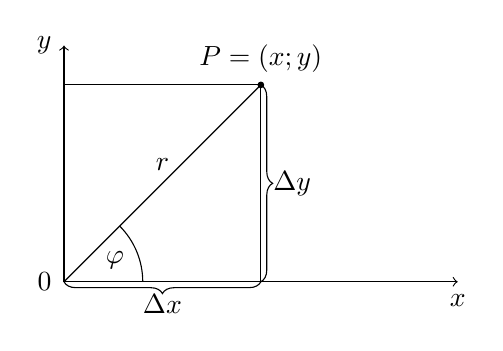
\begin{tikzpicture}
%Diagramm
  \draw [->] (0,0) -> (0,3cm)node[left=1pt]{$y$};
  \draw [->] (0,0)--(5cm,0)node[below=1pt]{$x$};
  \draw (0,0) node[left=1pt]{0};
%Koordinatensystem Punkt
  \draw ++(0,2.5cm)--++(2.5,0)--+(0,-2.5);
  \filldraw (2.5,2.5) circle (1pt);
  \draw (2.5,2.5cm)node[above=1pt]{$P=(x;y)$};
%Klammern
\begin{scope}[decoration={brace,amplitude=1.5mm}]
   \draw[decorate] (2.5,0) --(0,0);
   \draw[decorate] (2.5,2.5) --(2.5,0);
\end{scope}
%Beschriftung der Klammern
\draw (1.25,0)node[below=1pt]{$\Delta x$};
\draw (2.5,1.25)node[right=1pt]{$\Delta y$};
%Polarzeug
\draw (0,0)--(2.5,2.5);
\draw (1cm,0) arc (0:45:1cm);
\draw (45:1.77cm)node[above=1pt]{$r$};
\draw (22.5:.7cm)node{$\varphi$};
 \end{tikzpicture}\end{center}
\end{minipage}
\vspace{4pt}

\bla{Polarkoordinaten  $\Rightarrow$ Kartesische Koordinaten}

\begin{shaded}
 \begin{align}
  x&=r\cdot \cos \varphi& y=&r\cdot\sin\varphi
 \end{align}
\end{shaded}


\bla{Kartesische Koordinaten $\Rightarrow$ Polarkoordinaten}

\begin{shaded}
 \begin{align}
  r&=\sqrt{x^2+y^2}& \varphi=&\tan^{-1}\left(\frac{y}{x}\right)
 \end{align}
\end{shaded}

\bla{Koordinatentransformation(Parallelverschiebung)}

\begin{shaded}
 \begin{equation}
    y=f(x)\Rightarrow\left.\begin{aligned}
                            x&=u+a\\
			    y&=v+b
                           \end{aligned}\right.\Rightarrow v=f(u+a)-b
 \end{equation}
\end{shaded}
$(a;b)$: Ursprung des neuen u,v Koordinatensystems, bezogen auf das alte x,y-System. 

\section{Gleichungen}
\subsection{Gleichungen \emph{n}-ten Grades}
\begin{shaded}
 \begin{equation}
  a_n\cdot x^n+a_{n-1}\cdot x^{n-1}+\ldots+a_1\cdot x+a_0=0\quad (a_n\neq0,a_k\in\mathbb{R})
 \end{equation}

\end{shaded}
\bla{Eigenschaften}
\begin{itemize}
 \item Die Gleichung besitzen maximal $n$ reelle Lösungen.
\item Es gibt genau $n$ komplexe Lösungen.
\item Für ungerades $n$ gibt es mindestens eine reelle Lösung.
\item Komplexe Lösungen treten immer Paarweise auf.
\item Es existieren nur Lösungsformeln bis $n\leq 4$. Für $n>4$ gibt es nur noch grafische oder numerische Lösungswege.
\item Wenn eine Nullstelle bekannt ist kann man die Gleichung um einen Grad verringern, indem man denn zugehörigen Linearfaktor $x -x_1$ abspaltet(Polynome Division).
\end{itemize}

\subsection{Lineare Gleichungen}
\begin{shaded}
 \begin{equation}
  a_1\cdot x+a_0=0 \Rightarrow x_1=-\frac{a_0}{a_1}\quad (a_1\neq 0)
 \end{equation}
\end{shaded}

\subsection{Quadratische Gleichungen}
\begin{shaded}
 \begin{equation}
  a_2\cdot x^2+a_1\cdot x+a_0=0\quad (a_2\neq0)
 \end{equation}
\end{shaded}

\bla{Normalform mit Lösung}
\begin{shaded}
 \begin{equation}
  x^2+p\cdot x+q=0\Rightarrow x_{1/2}=-\frac{p}{2}\pm\sqrt{\left(\frac{p}{2}\right)^2-q}
 \end{equation}
\end{shaded}

\bla{Überprüfung (Vietascher Wurzelsatz)}
\begin{shaded}
 \begin{align}
  x_1+x_2&=-p& x_1\cdot x_2&=q 
 \end{align}
\end{shaded}
$x_1, x_2:$ Lösung der quadratischen Gleichung.

\subsection{Biquadratische Gleichungen}
Diese Gleichungen lassen sich mithilfe der Substitution lösen.
\begin{shaded}
 \begin{align}
  a\cdot x^4+b\cdot x^2 +c&=0&u&=x^2 \\
  a\cdot u^2+b\cdot u +c&=0&x&=\pm\sqrt{u}
 \end{align}
\end{shaded}
Das $u$ kann mithilfe der Lösungsformel einer quadratischen Gleichung gelöst werden.

\subsection{Gleichungen höheren Grades} 
Gleichungen höheren Grades kann man durch graphische oder numerische Ansätze lösen. Hilfreich ist das finden einer Lösung und das abspalten eines Linearfaktor
, mithilfe der Polynomendivision oder dem Hornor Schema,von der ursprünglichen Gleichung.

\bla{Polynomendivision}
\begin{shaded}
 \begin{equation}
  \frac{f(x)}{x-x_0}=\frac{a_3\cdot x^3+a_2\cdot x^2+a_1\cdot x +a_0}{x-x_0}=b_2\cdot x^2+b_1 \cdot x+b_0+r(x)
 \end{equation}
\end{shaded}
$x_0$ ist dabei die erste gefunden Nullstelle. r(x) verschwindet wenn $x_0$ ein Nullstellen oder eine Lösung von f(x) ist.
\begin{shaded}
 \begin{equation}
  r(x)=\frac{a_3\cdot x_0^3+a_2\cdot x_0^2+a_1\cdot x_0 +a_0}{x-x_0}=\frac{f(x_0)}{x-x_0}
 \end{equation}
\end{shaded}

\bla{Hornor-Schema}

\noindent\begin{tabularx}{\linewidth}{l|lllX}
\toprule
& $a_3$ & $a_2$ & $a_1$ & $a_0$\\
\midrule
\heboxc{$x_0$} & & $a_3\cdot x_0$ & $(a_2+a_3\cdot x_0)\cdot x_0$ &$(a_1+a_2\cdot x_0 +a_3\cdot x_0^2)\cdot x_0$ \\
& \heboxc{$a_3$} & $a_2+a_3\cdot x_0$ & $a_1+a_2\cdot x_0 + a_3\cdot x_0^2$ & $a_0+a_1\cdot x_0+a_2\cdot x_0^2+a_3\cdot x_0^3$\\
\midrule
& $b_2$ & $b_1$ & $b_0$& $f(x_0)$ \\
\bottomrule
\end{tabularx}
\subsection{Wurzelgleichung}
Wurzelgleichungen löst man durch quadrieren oder mit hilfe von Substitution.
Bei Wurzelgleichung ist zu beachten das quadrieren keine Aquivalente Umformung ist und das 
Ergebniss überprüft werden muss.

\subsection{Ungleichungen}
\begin{itemize*}
\item Beidseitiges Subtrahieren oder Addieren ist möglich
\item Die Ungleichung darf mit einer beliebige positiven Zahl multipliziert oder dividiert werden
\item Die Ungleichung darf mit einer beliebige negativen Zahl multipliziert oder dividiert werden, wenn man gleichzeitig das Relationszeichen umdreht.
\end{itemize*}

\subsection{Betragsgleichungen}
Betragsgleichungen löst man mithilfe der Fallunterscheidung. Dabei wird einmal davon ausgegangen das der Term inerhalb des Betrags einmal positiv und einmal negativen
sein kann.   
\begin{shaded}
\begin{equation}
y=|x|=\left\{
\begin{aligned}
  &x \\
- &x 
\end{aligned}
\right. \text{für} \left. \begin{aligned}
x &\geq 0 \\
x &< 0 
\end{aligned} \right\} 
\end{equation}
\end{shaded}

\subsection{Interpolationspolynome}
Entwicklung einer Polynomefunktion anhand von $n+1$ Kurvenpunkten.
\begin{description*}
 \item[1. Möglichkeit] Aufstellen von $n+1$ Gleichungen und ermitteln der Kurvenfunktion mithilfe des Gaußen Algorithmus.
 \item[2. Möglichkeit] Interpolationspolynome von Newton
\end{description*}

\bla{Interpolationspolynome von Newton}

\begin{merkbox}Gegeben sind die Punkte $P_0=(x_0;y_0)$, $P_1=(x_1;y_1)$, $P_2=(x_2;y_2)$, $\ldots$, $P_n=(x_n;y_n)$, damit lautet die Funktion wie folgt:
\begin{align}
 f(x)=a_0&+a_1\cdot (x-x_0)+ a_2\cdot (x-x_0)\cdot(x-x_1)\\
	 &+a_3\cdot(x-x_0)\cdot(x-x_1)\cdot(x-x_2)\\
	 &+\ldots\\
	 &+a_n\cdot(x-x_0)\cdot\ldots\cdot\cdot(x-x_{n-1})
\end{align}
Die Koeffizienten$a_0, a_1, a_2,\ldots, a_n$ lassen sich mithilfe des Differentenshema berechnen. Dabei ist $y_0=a_0$, $[x_0,x_1]=a_1$, $[x_0,x_1,x_2]=a_2$
 usw. 
\end{merkbox}

\bla{Differentenshema}

\noindent\begin{tabularx}{\linewidth}{cccccccX}
\toprule
 k	&$x_k$	&$y_k$		&$1$		&$2$		&$3$			&$\ldots$	\\ \midrule
 $0$	&$x_0$	&\hebox{$y_0$}	&		&		&			&		\\
	&	&		&\hebox{$[x_0,x_1]$}	&		&			&		\\
 $1$	&$x_1$	&$y_1$		&		&\hebox{$[x_0,x_1,x_2]$}&			&		\\
 	&	&		&$[x_1,x_2]$	&		&\hebox{$[x_0,x_1,x_2,x_3]$}	&		\\
 $2$	&$x_2$	&$y_2$		&		&\heboxc{$[x_1,x_2,x_3]$}&			&$\ldots$	\\
 	&	&		&$[x_2,x_3]$	&		&\heboxc{$[x_1,x_2,x_3,x_4]$}	&		\\
 $3$	&$x_3$	&$y_3$		&		&\heboxc{$[x_2,x_3,x_4]$}&			&$\ldots$	\\
 	&	&		&$\ldots$	&		&$\ldots$		&		\\
 $\vdots$&$\vdots$&$\vdots$	&		&		&			&		\\
 $n$	&$x_n$	&$y_n$		&		&		&			&		\\ \bottomrule
\end{tabularx}

\bla{Rechenregel für dividierte Differenzen}
\begin{shaded}
\begin{minipage}{.5\textwidth}

 \begin{equation}
 \left.\begin{aligned}
  [x_0,x_1]&=\frac{y_0-y_1}{x_0-x_1}\\
  [x_1,x_2]&=\frac{y_1-y_2}{x_1-x_2} \\
\vdots &
 \end{aligned}\right.
\end{equation} 
\end{minipage}\begin{minipage}{.5\textwidth}
 \begin{equation}
 \left.\begin{aligned}
  [x_0,x_1,x_2]&=\frac{[x_0,x_1]-[x_1,x_2]}{x_0-x_2}\\
  [x_1,x_2,x_3]&=\frac{[x_1,x_2]-[x_2,x_3]}{x_1-x_3} \\
\vdots &
 \end{aligned}\right.
\end{equation} 

\end{minipage}\end{shaded}
\begin{shaded}
 \begin{equation}
 \left.\begin{aligned}
  [x_0,x_1,x_2,x_3]&=\frac{[x_0,x_1,x_2]-[x_1,x_2,x_3]}{x_0-x_2}\\
  [x_1,x_2,x_3,x_4]&=\frac{[x_1,x_2,x_3]-[x_2,x_3,x_4]}{x_1-x_3} \\
\vdots &
 \end{aligned}\right.
\end{equation} 
\end{shaded}

\section{Komplexe Zahlen}
\begin{boxleft}\bla{Grundlagen}
\end{boxleft}\begin{boxrightshaded}
 \begin{align} 
j&=\sqrt{-1}\\
j^2&=-1
\end{align}\end{boxrightshaded}

\subsection{Darstellungsformen}

\begin{boxleft}\bla{Kartesische Form}
  \des[]{x}{Realanteil}\\
  \des[]{y}{Imaginäranteil}
\end{boxleft}\begin{boxrightshaded}
 \begin{align} 
z&=x+jy
\end{align}\end{boxrightshaded}

\begin{boxleft}
  \bla{Trigometrische Form}
\des[]{r}{Betrag}\\
\des[]{\varphi}{Argument}
\end{boxleft}\begin{boxrightshaded}
 \begin{align} 
z&=r\left(\cos{\varphi}+j\sin{\varphi}\right)
\end{align}\end{boxrightshaded}

\begin{boxleft}
  \bla{Exponentialform}
\end{boxleft}\begin{boxrightshaded}
 \begin{align} 
z&=re^{j\varphi}
\end{align}\end{boxrightshaded}

\begin{boxleft}
  \bla{Umrechnung}
\end{boxleft}\begin{boxrightshaded}
 \begin{align} 
x&=r\cos{\varphi}\\
y&=r\sin{\varphi}\\
r&=\left|z\right|=\sqrt{x^2+y^2}
\end{align}\end{boxrightshaded}

\begin{boxleft}
  \bla{Umrechnung Winkel}
\end{boxleft}\begin{boxrightshaded}
 \begin{align} 
\tan{\varphi}&=\frac{y}{x}\\
\varphi&=\begin{dcases*}
  \arctan{\frac{y}{x}}& Quadrant I\\
\arctan{\frac{y}{x}}+\pi& Quadrant II,III\\
\arctan{\frac{y}{x}}+2\pi& Quadrant IV
\end{dcases*}
\end{align}\end{boxrightshaded}

\subsection{Rechenregeln}

\begin{boxleft}
  \bla{Konjugiert komplexe Zahl}
\des[]{\overline{z}}{konjugierte Komplexe}
\end{boxleft}\begin{boxrightshaded}
 \begin{align} 
\overline{z}&=z^*\\
\overline{z}&=\overline{x+jy}\\
&=x-jy\\
\overline{z}&=\overline{r\left(\cos{\varphi}+j\sin{\varphi}\right)}\\
&=r\left(\cos{\varphi}-j\sin{\varphi}\right)\\
\overline{z}&=\overline{re^{j\varphi}}\\
&=re^{-j\varphi}
\end{align}\end{boxrightshaded}

\begin{boxleft}\bla{Addition und Subtraktion}
\end{boxleft}\begin{boxrightshaded}
\begin{align} 
  z_1\pm z_2&=(x_1+jy_1)\pm(x_2+jy_2)\\
	    &=(x_1\pm x_2)+ j(y_1 \pm y_2)
\end{align}\end{boxrightshaded}

\begin{boxleft}\bla{Multiplikation}
\end{boxleft}\begin{boxrightshaded}
\begin{align} 
 z_1 \cdot z_2&=(x_1+jy_1)\cdot(x_2+jy_2)\\
	      &=(x_1x_2-y_1y_2)+ j(x_1y_2+x_2y_1)\\
 z_1 \cdot z_2&=r_1\left(\cos{\varphi_1}+j\sin{\varphi_1}\right)\cdot r_2\left(\cos{\varphi_2}+j\sin{\varphi_2}\right)\\
	      &=r_1r_2\left(\cos(\varphi_1+\varphi_2)+j\sin(\varphi_1+\varphi_2)\right)\\
 z_1 \cdot z_2&=r_1e^{j\varphi_1}\cdot r_2e^{j\varphi_2}\\
	      &=r_1r_2e^{j(\varphi_1+\varphi_2)}
\end{align}\end{boxrightshaded}

\begin{boxleft}\bla{Division}
\end{boxleft}\begin{boxrightshaded}
\begin{align} 
\frac{z_1}{z_2} &=\frac{x_1+jy_1}{x_2+jy_2}\\
		&=\frac{x_1x_2+y_1y_2}{x_2^2+y_2^2}+j\frac{x_2y_1-x_1y_2}{x_2^2+y_2^2}\\
\frac{z_1}{z_2} &=\frac{r_1\left(\cos{\varphi_1}+j\sin{\varphi_1}\right)}{r_2\left(\cos{\varphi_2}+j\sin{\varphi_2}\right)}\\
	        &=\frac{r_1}{r_2}\left(\cos(\varphi_1-\varphi_2)+j\sin(\varphi_1-\varphi_2)\right)\\
\frac{z_1}{z_2} &=\frac{r_1e^{j\varphi_1}}{r_2e^{j\varphi_2}}\\
	        &=\frac{r_1}{r_2}e^{j(\varphi_1-\varphi_2)}
\end{align}\end{boxrightshaded}

\begin{boxleft}\bla{Potenzieren}
\end{boxleft}\begin{boxrightshaded}
\begin{align} 
z^n		&=\left(r_1\left(\cos{\varphi_1}+j\sin{\varphi_1}\right)\right)^n\\
		&=r_1^n\left(\cos(n\varphi_1)+j\sin(n\varphi_1)\right)\\
z^n		&=\left(r_1e^{j\varphi_1}\right)^n\\
		&=r_1^ne^{jn\varphi_1}
\end{align}\end{boxrightshaded}

\begin{boxleft}\bla{Wurzelziehen}
\destext{Es entsthen n Lösungen}\\
\destext{Für k muss nacheinander $0,1,\dots,n-1$ eingesetzt werden}
\end{boxleft}\begin{boxrightshaded}
\begin{align} 
\sqrt[n]{z}	&=\sqrt[n]{r_1\left(\cos\varphi_1+j\sin{\varphi_1}\right)}\\
\omega_k	&=\sqrt[n]{r_1}\left(\cos\left(\frac{\varphi_1+2k\pi}{n}\right)+j\sin\left(\frac{\varphi_1+2k\pi}{n}\right)\right)\\
\sqrt[n]{z}	&=\sqrt[n]{r_1e^{j\varphi_1}}\\
\omega_k	&=\sqrt[n]{r_1}e^{j\left(\frac{\varphi_1+2k\pi}{n}\right)}
\end{align}\end{boxrightshaded}
\section{Differntialrechnung}

\subsection{Erste Ableitung der elementaren Funktionen}
\begin{boxleft}
  \bla{Potenzfunktion}
\end{boxleft}\begin{boxrightshaded}
 \begin{align}
  &x^n& 	&n\cdot x^{n-1}
 \end{align}
\end{boxrightshaded}

\begin{boxleft}
  \bla{Exponentialfunktionen}
\end{boxleft}\begin{boxrightshaded} \begin{align}
  &e^x& 	&e^x\\
  &a^x& 	&\ln a\cdot a^x
 \end{align}
\end{boxrightshaded}

\begin{boxleft}
  \bla{Logarithmusfunktionen}
\end{boxleft}\begin{boxrightshaded}
 \begin{align} 
  &\ln x& &\frac{1}{x}\\
  &\log_a x&	&\frac{1}{(\ln a)\cdot x}
 \end{align}
\end{boxrightshaded}

\begin{boxleft}
  \bla{Trigonometrische Funktionen}
\end{boxleft}\begin{boxrightshaded}
 \begin{align} 
  &\sin x& 	&\cos x \\
  &\cos x& 	&-\sin x\\
  &\tan x&	&\frac{1}{\cos^2 x}\\
  &\tan x&	&1+\tan^2 x
\end{align}\end{boxrightshaded}
 
\begin{boxleft}
  \bla{Arcusfunktionen}
\end{boxleft}\begin{boxrightshaded}
 \begin{align} 
  &\arcsin x& &\frac{1}{\sqrt{1-x^2}}\\
  &\arccos x& &\frac{-1}{\sqrt{1-x^2}}\\
  &\arctan x& &\frac{1}{1-x^2}
\end{align}\end{boxrightshaded}

\begin{boxleft}
  \bla{Hyperbelfunktionen}
\end{boxleft}\begin{boxrightshaded}
 \begin{align} 
  &\sinh x& &\cosh x\\
  &\cosh x& &\sinh x\\
  &\tanh x& &\frac{1}{\cosh^2 x}\\
  &\tanh x& &1+\tanh^2 x
\end{align}\end{boxrightshaded}
          
\subsection{Rechenregeln}

\begin{boxleft}
  \bla{Faktorregel}
\end{boxleft}\begin{boxrightshaded}
 \begin{align} 
\frac{\diff }{\diff x}\left(C\cdot f(x)\right)=C\cdot f'(x)
 \end{align}\end{boxrightshaded}

\begin{boxleft}
  \bla{Summenregel}
\end{boxleft}\begin{boxrightshaded}
 \begin{align} 
\frac{\diff }{\diff x}\left(g(x) + f(x)\right)=g'(x)+f'(x)
 \end{align}\end{boxrightshaded}

\begin{boxleft}
  \bla{Produktregel}
\end{boxleft}\begin{boxrightshaded}
 \begin{align} 
\frac{\diff }{\diff x}&\left(g(x)\cdot f(x)\right)=g'(x)\cdot f(x)+g(x)\cdot f'(x)\\
\frac{\diff }{\diff x}&\left(h(x)\cdot g(x)\cdot f(x)\right)=h'\cdot g\cdot f+h\cdot g'\cdot f+h\cdot g\cdot f'
 \end{align}\end{boxrightshaded}
            
\begin{boxleft}
  \bla{Quotientenregel}
\end{boxleft}\begin{boxrightshaded}
 \begin{align} 
\frac{\diff }{\diff x}\left(\frac{g(x)}{f(x)}\right)&=\frac{g'(x)\cdot f(x)-g(x)\cdot f'(x)}{f(x)^2}
 \end{align}\end{boxrightshaded}
            
\begin{boxleft}
  \bla{Kettenregel}
\end{boxleft}\begin{boxrightshaded}
 \begin{align} 
\frac{\diff }{\diff x}\left(g\left( f(x\right)\right)&=g'(f)\cdot f'(x)
 \end{align}\end{boxrightshaded}
                 
\begin{boxleft}
  \bla{Logarithmische Ableitungen}
\end{boxleft}\begin{boxrightshaded}
 \begin{align} 
\frac{\diff }{\diff x}y&=f(x)\\
\frac{1}{y}y'&=\frac{\diff }{\diff x}\ln{f(x)}
 \end{align}\end{boxrightshaded}
                   
\subsection{Fehlerrechnung}

\begin{boxleft}\bla{Absolute Fehler}
\des[]{\Delta x}{Absoluter Fehler der Eingangsgröße}\\
\des[]{\Delta y}{Absoluter Fehler der Ausgangsgröße}
\end{boxleft}\begin{boxrightshaded}
\begin{align} 
\Delta y=f(x+\Delta x)-f(x)
\end{align}\end{boxrightshaded}
         
\begin{boxleft}\bla{Relativer Fehler}
\des[]{\delta x}{Relativer Fehler der Eingangsgröße in $\%$}\\
\des[]{\delta y}{Relativer Fehler der Ausgangsgröße in $\%$}
\end{boxleft}\begin{boxrightshaded}
\begin{align} 
\delta x&=\frac{\Delta x}{x}\\
\delta y&=\frac{\Delta y}{y}\\
\Delta y&=f'(x)\cdot \Delta x\\
\delta y&=\frac{x\cdot f'(x)}{f(x)}\delta x
\end{align}\end{boxrightshaded}
         
\subsection{Linearisierung und Taylor-Polynome}

\begin{boxleft}\bla{Tangentengleichung}
\des[]{x_0}{Punkt an denn das Polynome entwickelt wird}
\end{boxleft}\begin{boxrightshaded}
\begin{align} 
y_T(x)&=f(x_0)+f'(x_0)(x-x_0)
\end{align}\end{boxrightshaded}

\begin{boxleft}\bla{Taylor Polynome}
\des[]{x_0}{Punkt an denn das Polynome entwickelt wird}\\
\des[]{R_n}{Restglied}
\end{boxleft}\begin{boxrightshaded}
\begin{align} 
y(x)&=f(x_0)+f'(x_0)(x-x_0)+\frac{f''(x_0)}{2!}(x-x_0)^2+\dots+\frac{f^{(n)}(x_0)}{n!}(x-x_0)^n+R_n(x)\\
    &=\sum_{i=0}^n\frac{f^{(i)}}{i!}(x-x_0)^i+R_n(x)
\end{align}\end{boxrightshaded}


\begin{boxleft}\bla{Restglied}
\des[]{x_0}{Punkt an denn das Polynome entwickelt wird}\\
\des[]{c}{$x_0<c<x$, wenn $x_0<x$}\\
\des[]{c}{$x_0>c>x$, wenn $x_0>x$}
\end{boxleft}\begin{boxrightshaded}
\begin{align} 
R_n(x)=\frac{f^{(n+1)}(c)}{(n+1)!}(x-x_0)^{n+1}
\end{align}\end{boxrightshaded}

\subsection{Grenzwertregel von Bernoulli und de l`Hospital}
\begin{boxleft}\bla{de l`Hospital}
\destext{Gilt nur wenn $\lim_{x \to x_0} f(x)$ gleich $\frac{0}{0}$ oder $\frac{\infty}{\infty}$ ist}
\end{boxleft}\begin{boxrightshaded}
\begin{align} 
 \lim_{x \to x_0}\frac{f(x)}{g(x)}=\lim_{x \to x_0}\frac{f'(x)}{g'(x)}
\end{align}\end{boxrightshaded}

\subsection{Differentielle Kurvenuntersuchung}


\begin{boxleft}\bla{Normale der Kurve}
\end{boxleft}\begin{boxrightshaded}
\begin{align} 
y_N(x)&=f(x_0)-\frac{1}{f'(x)}\left(x-x_0\right)
\end{align}\end{boxrightshaded}

\begin{boxleft}\bla{Monotonie-Verhalten}
\end{boxleft}\begin{boxrightshaded}
\begin{align} 
f'(x)&>0&&\text{Monoton wachsend}\\
f'(x)&<0&&\text{Monoton fallend} 
\end{align}\end{boxrightshaded}

\begin{boxleft}\bla{Krümmung-Verhalten}
\end{boxleft}\begin{boxrightshaded}
\begin{align} 
f''(x)&>0&&\text{Linkskrümmung(konvex)}\\
f''(x)&<0&&\text{Rechtskrümmung(konkav)} 
\end{align}\end{boxrightshaded}

\begin{boxleft}\bla{Ableitung Polarkordinaten}
\des[]{\dot{r}}{Ableitung nach $\varphi$}\\
\des[]{\ddot{r}}{Zweite Ableitung nach $\varphi$}
\end{boxleft}\begin{boxrightshaded}
\begin{align} 
y(\varphi)&=r(\varphi)\sin\varphi\\
x(\varphi)&=r(\varphi)\cos\varphi\\
y'&=\frac{\diff y}{\diff x}=\frac{r'\sin\varphi+r\cos\varphi}{r'\cos\varphi-r\sin\varphi}\\
y''&=\frac{\diff^2 y}{\diff x^2}=\frac{2(r')^2-r\cdot r''+r^2}{\left(r'\cos\varphi-r\sin\varphi\right)^3}
\end{align}\end{boxrightshaded}

\begin{boxleft}\bla{Ableitung Parameterform}
\des[]{\dot{x}}{Ableitung nach t}\\
\des[]{\dot{y}}{Ableitung nach t}
\end{boxleft}\begin{boxrightshaded}
\begin{align} 
y&=y(t)\\
x&=x(t)\\
y'&=\frac{\diff y}{\diff x}=\frac{\dot{y}}{\dot{x}}\\
y''&=\frac{\diff^2 y}{\diff x^2}=\frac{\dot{x}\ddot{y}-\dot{y}\ddot{x}}{\dot{x}^3}
\end{align}\end{boxrightshaded}

\begin{boxleft}\bla{Ableitung Parameterform}
\des[]{\dot{x}}{Ableitung nach t}\\
\des[]{\dot{y}}{Ableitung nach t}
\end{boxleft}\begin{boxrightshaded}
\begin{align} 
y&=y(t)\\
x&=x(t)\\
y'&=\frac{\diff y}{\diff x}=\frac{\dot{y}}{\dot{x}}\\
y''&=\frac{\diff^2 y}{\diff x^2}=\frac{\dot{x}\ddot{y}-\dot{y}\ddot{x}}{\dot{x}^3}
\end{align}\end{boxrightshaded}

\begin{boxleft}\bla{Bogendifferential}
\destext{"Wegelement" einer Funktion}
\end{boxleft}\begin{boxrightshaded}
\begin{align} 
\diff s&=\sqrt{1+\left(f'(x)\right)^2}\cdot \diff x\\
\diff s&=\sqrt{(\dot{x})^2+(\dot{y})^2}\cdot \diff t\\
\diff s&=\sqrt{r^2+(r')^2}\cdot \diff \varphi
\end{align}\end{boxrightshaded}

\begin{boxleft}\bla{Winkeländerung}
\end{boxleft}\begin{boxrightshaded}
\begin{align} 
\tau&=\arctan y'\\
\diff \tau&=\frac{y''}{1+(y')^2}\cdot \diff x
\end{align}\end{boxrightshaded}

\begin{boxleft}\bla{Kurvenkrümmung}
\end{boxleft}\begin{boxrightshaded}
\begin{align} 
\kappa&=\frac{\diff \tau}{\diff s}\\
\kappa&=\frac{y''}{\sqrt{\left(1+(y')^2\right)^3}}\\
\kappa&=\frac{\dot{x}\ddot{y}-\dot{y}\ddot{x}}{\sqrt{\left(\dot{x}^2+\dot{y}^2\right)^3}}\\
\kappa&=\frac{2(r')^2-r\cdot r''+r^2}{\sqrt{\left(r^2+(r')^2\right)^3}}
\end{align}\end{boxrightshaded}

\begin{boxleft}\bla{Krümmungskreis}
\des[]{\rho}{Radius des Krümmungskreises}\\
\des[]{x_K}{x-Koordinaten des Kreismittelpunktes}\\
\des[]{y_K}{y-Koordinaten des Kreismittelpunktes}\\
\des[]{x_P}{x-Koordinaten des Kurvenpunktes}\\
\des[]{y_P}{y-Koordinaten des Kurvenpunktes}
\end{boxleft}\begin{boxrightshaded}
\begin{align} 
\rho&=\frac{1}{|\kappa|}\\
x_K&=x_P-y'\frac{1+(y')^2}{|y''|}\\
y_K&=y_P+\frac{1+(y')^2}{|y''|}
\end{align}\end{boxrightshaded}





\section{Vektorrechnung}
\subsection{Grundlagen}

\begin{boxleft}\bla{Darstellung}
\end{boxleft}\begin{boxrightshaded}
\begin{align} 
\vv{a}	&=\vv{a}_x+\vv{a}_y+\vv{a}_z\\
	&=a_x\vv{e}_x+a_y\vv{e}_y+a_y\vv{e}_y\\
	&=\begin{pmatrix} a_x\\ a_y\\a_z\end{pmatrix}
\end{align}\end{boxrightshaded}

\begin{boxleft}\bla{2 Punkt Vektor}
\end{boxleft}\begin{boxrightshaded}
\begin{align} 
\vv{P_1P_2} &=\begin{pmatrix} x_2-x_1\\ y_2-y_1\\z_2-z_1\end{pmatrix}
\end{align}\end{boxrightshaded}

\begin{boxleft}\bla{Betrag}
\end{boxleft}\begin{boxrightshaded}
\begin{align} 
|\vv{a}|	&=a\\
		&=\sqrt{a_x^2+a_y^2+a_z^2}\\
		&=\sqrt{\vv{a}\circ\vv{a}}
\end{align}\end{boxrightshaded}

\begin{boxleft}\bla{Richtungswinkel}
\end{boxleft}\begin{boxrightshaded}
\begin{align} 
\cos \alpha &= \frac{a_x}{|\vv{a}|}\\
\cos \beta &= \frac{a_y}{|\vv{a}|}\\
\cos \gamma &= \frac{a_z}{|\vv{a}|}\\
1&=\cos^2\alpha+\cos^2\beta+\cos^2\gamma
\end{align}\end{boxrightshaded}

\subsection{Vektoroperationen}

\begin{boxleft}\bla{Addition und Subtraktion}
\end{boxleft}\begin{boxrightshaded}
\begin{align} 
\vv{a}\pm\vv{b}&= \begin{pmatrix}a_x\pm b_x\\a_y\pm b_y\\a_z\pm b_z\end{pmatrix}
\end{align}\end{boxrightshaded}

\begin{boxleft}\bla{Multiplikation mit einem Skalar}
\end{boxleft}\begin{boxrightshaded}
\begin{align} 
a\cdot\vv{b}&= \begin{pmatrix}ab_x\\ ab_y\\ab_z\end{pmatrix}
\end{align}\end{boxrightshaded}

\begin{boxleft}\bla{Einheitsvektor}
\end{boxleft}\begin{boxrightshaded}
\begin{align} 
\vv{e}_a&=\frac{\vv{a}}{|\vv{a}|}= \begin{pmatrix}a_x/|\vv{a}|\\ a_y/|\vv{a}|\\a_z/|\vv{a}|\end{pmatrix}
\end{align}\end{boxrightshaded}

\begin{boxleft}\bla{Skalarprodukt}
\end{boxleft}\begin{boxrightshaded}
\begin{align} 
\vv{a}\circ\vv{b} &= \begin{pmatrix}a_x\\ a_y\\a_z\end{pmatrix}\circ\begin{pmatrix}b_x\\ b_y\\b_z\end{pmatrix}=a_xb_x+a_yb_y+a_zb_z\\
		  &=|\vv{a}|\cdot|\vv{b}|\cdot \cos\angle(\vv{a},\vv{b})
\end{align}\end{boxrightshaded}

\begin{boxleft}\bla{Kreuzprodukt}
\destext{$|\vv{a}\times\vv{b}|$ Fläche des Parallelograms $\vv{a},\vv{b}$}\\
\destext{$\vv{a}\times\vv{b} \perp \vv{a} \land \vv{a}\times\vv{b} \perp \vv{b}$}
\end{boxleft}\begin{boxrightshaded}
\begin{align} 
\vv{a}\times\vv{b} &= \begin{pmatrix}a_x\\ a_y\\a_z\end{pmatrix}\times\begin{pmatrix}b_x\\ b_y\\b_z\end{pmatrix}=\begin{pmatrix}a_yb_z-a_zb_y\\ a_zb_x-a_xb_z\\a_xb_y-a_yb_x\end{pmatrix}\\
		  &=\begin{vmatrix}\vv{e}_x&\vv{e}_y&\vv{e}_z\\a_x&a_y&a_z\\b_x&b_y&b_z\end{vmatrix}
\end{align}\end{boxrightshaded}

\begin{boxleft}\bla{Spatprodukt}
\destext{$\vv{a}\circ(\vv{b}\times\vv{c})$ Volumen des Parallelpiped $\vv{a},\vv{b},\vv{c}$}
\end{boxleft}\begin{boxrightshaded}
\begin{align} 
[\vv{a}\vv{b}\vv{c}]  &=\vv{a}\circ(\vv{b}\times\vv{c})\\
		      &=a_x(b_yc_z-b_zc_y)+a_y(b_zc_x-b_xc_z)+a_z(b_xc_y-b_yc_x)\\
		      &=\begin{vmatrix}a_x&a_y&a_z\\b_x&b_y&b_z\\c_x&c_y&c_z\end{vmatrix}
\end{align}\end{boxrightshaded}

\begin{boxleft}\bla{Schnittwinkel}
\end{boxleft}\begin{boxrightshaded}
\begin{align} 
\cos\angle(\vv{a},\vv{b})&=\frac{\vv{a}\circ\vv{b}}{|\vv{a}|\cdot|\vv{b}|}
\end{align}\end{boxrightshaded}

\begin{boxleft}\bla{Projektion}
\end{boxleft}\begin{boxrightshaded}
\begin{align} 
\vv{a}_b&=\left(\frac{\vv{a}\circ\vv{b}}{|\vv{a}|^2}\right)\vv{a}=(\vv{b}\circ\vv{e}_a)\vv{e}_a
\end{align}\end{boxrightshaded}

\subsection{Geraden}


\begin{boxleft}\bla{Geradegleichung}
\des[]{\vv{r}_1}{Ortsvektor (Verschiebung von Ursprung)}\\
\des[]{\vv{a}}{Richtungsvektor}
\end{boxleft}\begin{boxrightshaded}
\begin{align} 
\vv{r}(t) &=\vv{r}_1+t\vv{a}\\
	  &=\vv{r}_1+t(\vv{r}_2-\vv{r}_1)
\end{align}\end{boxrightshaded}

\begin{boxleft}\bla{Abstand eines Punktes von einer Geraden}
\des[]{\vv{r}_1}{Ortsvektor (Verschiebung von Ursprung)}\\
\des[]{\vv{a}}{Richtungsvektor}\\
\des[]{\vv{OP}}{Ortsvektor des Punktes P}
\end{boxleft}\begin{boxrightshaded}
\begin{align} 
\vv{r}(t) &=\vv{r}_1+t\vv{a}\\
d&=\frac{|\vv{a}\times\left(\vv{OP}-\vv{r}_1\right)|}{\vv{a}}
\end{align}\end{boxrightshaded}

\begin{boxleft}\bla{Abstand zweier paralleler Geraden}
\des[]{\vv{r}_1}{Ortsvektor der ersten Gerade}\\
\des[]{\vv{r}_2}{Ortsvektor der zweiten Gerade}\\
\des[]{\vv{a}_1}{Richtungsvektor der Geraden}
\end{boxleft}\begin{boxrightshaded}
\begin{align} 
\vv{r}(t) &=\vv{r}_1+t\vv{a}_1\\
\vv{g}(t) &=\vv{r}_2+t\vv{a}_1\\
d&=\frac{|\vv{a}_1\times\left(\vv{r}_2-\vv{r}_1\right)|}{\vv{a}_1}
\end{align}\end{boxrightshaded}


\begin{boxleft}\bla{Abstand zweier windschiefen Geraden}
\des[]{\vv{r}_1}{Ortsvektor der ersten Gerade}\\
\des[]{\vv{r}_2}{Ortsvektor der zweiten Gerade}\\
\des[]{\vv{a}_1}{Richtungsvektor der ersten Geraden}\\
\des[]{\vv{a}_2}{Richtungsvektor der zweiten Geraden}
\end{boxleft}\begin{boxrightshaded}
\begin{align} 
\vv{r}(t) &=\vv{r}_1+t\vv{a}_1\\
\vv{g}(t) &=\vv{r}_2+t\vv{a}_2\\
d&=\frac{|\vv{a}_1\circ\left(\vv{a}_2\times\left(\vv{r}_2-\vv{r}_1\right)\right)|}{\vv{a}_1\times\vv{a}_2}
\end{align}\end{boxrightshaded}

\subsection{Ebenen}

\begin{boxleft}\bla{Ebenengleichung}
\des[]{\vv{r}_1}{Ortsvektor der Ebenen}\\
\des[]{\vv{a}_1}{Erster Richtungsvektor}\\
\des[]{\vv{a}_2}{Zweiter Richtungsvektor}
\end{boxleft}\begin{boxrightshaded}
\begin{align} 
\vv{r}(t,s) &=\vv{r}_1+t\vv{a}_1+s\vv{a}_2\\
	    &=\vv{r}_1+t(\vv{r}_2-\vv{r}_1)+s(\vv{r}_3-\vv{r}_1)
\end{align}\end{boxrightshaded}

\begin{boxleft}\bla{Normalenvektor}
\des[]{\vv{n}}{Normalenvektor}\\
\des[]{\vv{r}_1}{Ortsvektor der Normalen}\\
\des[]{\vv{r}}{$(x,y,z)^T$}
\end{boxleft}\begin{boxrightshaded}
\begin{align} 
\vv{n}\circ\left(\vv{r}-\vv{r}_1\right)=0
\end{align}\end{boxrightshaded}

\begin{boxleft}\bla{Normalenvektor}
\des[]{\vv{n}}{Normalenvektor}\\
\des[]{\vv{r}_1}{Ortsvektor der Normalen}\\
\des[]{\vv{r}}{$(x,y,z)^T$}
\end{boxleft}\begin{boxrightshaded}
\begin{align} 
0&=\vv{n}\circ\left(\vv{r}-\vv{r}_1\right)\\
\vv{n}&=\vv{a}_1\times\vv{a}_2
\end{align}\end{boxrightshaded}

\begin{boxleft}\bla{Parameterfreie Darstellung}
\des[]{\vv{n}}{Normalenvektor}
\end{boxleft}\begin{boxrightshaded}
\begin{align} 
\vv{r}(t,s) &=\vv{r}_1+t\vv{a}_1+s\vv{a}_2\\
\vv{r}\circ(\vv{a}_1\times\vv{a}_2)&=\vv{r}_1\circ(\vv{a}_1\times\vv{a}_2)+t\vv{a}_1\circ(\vv{a}_1\times\vv{a}_2)\\
&\qquad +s\vv{a}_2\circ(\vv{a}_1\times\vv{a}_2)\\
\vv{r}\circ\vv{n}&=\vv{r}_1\circ\vv{n}+0+0
\end{align}\end{boxrightshaded}

\begin{boxleft}\bla{Normierter Normalenvektor}
\end{boxleft}\begin{boxrightshaded}
\begin{align} 
\vv{e}_n&=\frac{\vv{a}_1\times\vv{a}_2}{|\vv{a}_1\times\vv{a}_2|}
\end{align}\end{boxrightshaded}

\begin{boxleft}\bla{Hesseschen Normalform}
\end{boxleft}\begin{boxrightshaded}
\begin{align} 
0&=\frac{Ax+By+Cz+D}{\sqrt{A^2+B^2+C^2}}
\end{align}\end{boxrightshaded}


\begin{boxleft}\bla{Abstand eines Punktes von einer Ebene}
\des[]{\vv{n}}{Normalenvektor}\\
\des[]{\vv{r}_1}{Ortsvektor der Normalen}\\
\des[]{\vv{OP}}{Ortsvektor des Punktes P}\\
\des[]{p_i}{Koordinaten des Punktes P}
\end{boxleft}\begin{boxrightshaded}
\begin{align} 
d&=\frac{|\vv{n}\times\left(\vv{OP}-\vv{r}_1\right)|}{\vv{n}}\\
d&=\frac{Ap_1+Bp_2+Cp_3+D}{\sqrt{A^2+B^2+C^2}}
\end{align}\end{boxrightshaded}


\begin{boxleft}\bla{Abstand eines Geraden von einer Ebene}
\des[]{\vv{n}}{Normalenvektor}\\
\des[]{\vv{r}_1}{Ortsvektor der Normalen}\\
\des[]{\vv{r}_G}{Ortsvektor der Geraden}\\
\des[]{r_{Gi}}{Koordinaten eines Geraden Punktes}
\end{boxleft}\begin{boxrightshaded}
\begin{align} 
\vv{r}(t) &=\vv{r}_G+t\vv{a}_1\\
d&=\frac{|\vv{n}\times\left(\vv{r}_G-\vv{r}_1\right)|}{\vv{n}}\\
d&=\frac{Ar_{G1}+Br_{G2}+Cr_{G3}+D}{\sqrt{A^2+B^2+C^2}}
\end{align}\end{boxrightshaded}


\begin{boxleft}\bla{Abstand zweier paralleler Ebenen}
\des[]{\vv{n}}{Normalenvektor}
\end{boxleft}\begin{boxrightshaded}
\begin{align} 
\vv{r}(t,s) &=\vv{r}_1+t\vv{a}_1+s\vv{a}_2\\
\vv{g}(t,s) &=\vv{r}_2+t\vv{a}_3+s\vv{a}_4\\
d&=\frac{|\vv{n}\times\left(\vv{r}_1-\vv{r}_2\right)|}{\vv{n}}
\end{align}\end{boxrightshaded}


\begin{boxleft}\bla{Schnittwinkel zweier Ebenen}
\destext{$\angle$ Ebenen = $\angle(\vv{n}_1,\vv{n}_2)$}
\end{boxleft}\begin{boxrightshaded}
\begin{align} 
\cos\angle(\vv{n}_1,\vv{n}_2)&=\frac{\vv{n}_1\circ\vv{n}_2}{|\vv{n}_1|\cdot|\vv{n}_2|}
\end{align}\end{boxrightshaded}

\begin{boxleft}\bla{Durchstoßpunkt}
\des[]{\vv{n}}{Normalenvektor}\\
\des[]{\vv{r}_1}{Ortsvektor der Normalen}\\
\des[]{\vv{r}_G}{Ortsvektor der Geraden}\\
\des[]{\vv{r}_s}{Ortsvektor des Schnittpunktes}
\end{boxleft}\begin{boxrightshaded}
\begin{align} 
\vv{r}(t) &=\vv{r}_G+t\vv{a}\\
\vv{r}_s&=\vv{r}_G+\frac{\vv{n}\circ\left(\vv{r}_1-\vv{r}_G\right)}{\vv{n}\circ\vv{a}}\vv{a}\\
\varphi&=\arcsin\left(\frac{|\vv{n}\circ\vv{a}|}{|\vv{n}|\cdot|\vv{a}|}\right)
\end{align}\end{boxrightshaded}
